% !TEX root = report.tex
%============================================================================================
\newpage
\section{Robust PCA with known rank: a block coordinate descent approach}

%-----------------------------------------------------------------------------------------------------------------------------------------------------------------
\subsection{Motivation}
In some application, we normally have some prior information about the low rank component of an observed matrix. For example, in computer vision, if we are to extract the background from different frames of a video, then it is natural to consider each video frame as a long vector. The background that we are recovering is then one vector, which is of rank 1. Therefore, it is natural to see if we can utilize this additional rank information to derive faster algorithms while retaining the performance guarantee.



%-----------------------------------------------------------------------------------------------------------------------------------------------------------------
\subsection{Equivalent formulation of Robust PCA with rank information}

We first show the intuitive fact that in the robust PCA framework, the same probability
guarantee will still hold when additional information on the problem is incorporated into the optimization problem. . Then we
derive a block-coordinate descent algorithm for the case when rank
information is known.
\begin{prop}
\label{prop:restriction prob}Let $M=L_{0}+S_{0}$ , $rank(L_{0})\le r$ and $(L_0,S_0)$
satisfy the Robust PCA assumptions. Then with high probability, the
following problems are equivalent:

\begin{eqnarray}
J_{1} & =\min_{L,S} & \|L\|_{*}+\lambda\|S\|_{1}\label{eq:general}\\
 & s.t. & M=L+S\nonumber
\end{eqnarray}

\begin{eqnarray}
J_{2} & =\min_{L,S} & \|L\|_{*}+\lambda\|S\|_{1}\label{eq:restricted}\\
 & s.t. & M=L+S\nonumber \\
 &  & \text{and }T(L,S)\text{ holds}\nonumber
\end{eqnarray}


where $T(L,S)$ are conditions on $(L,S)$ that $(L_{0},S_{0})$ also
satisfies.
\end{prop}

\begin{proof}
We use subscript to denote the optimizer for $J_{1}$ and $J_{2}$ respectively.
With high probability, $(L_{1},S_{1})=(L_{0},S_{0})$. Now, over the event of $(L_{1},S_{1})=(L_{0},S_{0})$, $(L_{1},S_{1})$ is also a feasible solution for (\ref{eq:restricted}). Since $J_{1}\le J_{2}$ always, now $(L_{1},S_{1})$ achieve the bound for (\ref{eq:restricted}).
Note that it should also be unique because otherwise it would contradict with the recovery of (\ref{eq:general}).
\end{proof}

Now we apply Proposition (\ref{prop:restriction prob}) to the case when the rank information is known and derive a block coordinate descent framework for future algorithm design.

\begin{alignat}{3}
J_{3} 
&= &&\min_{L, S}  && \|L\|_{*} + \lambda \|S\|_{1} \notag \\
&&&\text{s.t.} && M=L+S, \ \text{rank}(L)\le r \notag \\
&= &&\min_{L, S, p_i, q_i, \mu_i} && \|L\|_{*} + \lambda\| M - L \|_{1} \notag \\
&&& \text{s.t.} && L = \sum_{i=1}^{r} \mu_{i}p_{i}q_{i}^{T}, \  \|p_{i}\|_{2}=1, \ \|q_{i}\|_{2}=1, \ \mu_{i}\ge0 \notag \\
&= && \min_{\mu_{i}, p_{i}, q_{i}} && \sum_{i=1}^{r} \mu_{i} + \lambda \|M - \sum_{i=1}^{r} \mu_{i}p_{i}q_{i}^{T}\|_{1} \notag \\
&&& \text{s.t.} && \|p_{i}\|_{2} = 1, \ \|q_{i}\|_{2} = 1, \mu_{i} \ge 0 \notag \\
& = && \min_{\mu_{i}, p_{i}, q_{i}} && \sum_{i=1}^{r} |\mu_{i}-0| + \lambda \|M - \sum_{i=1}^{r} \mu_{i} p_{i} q_{i}^{T}\|_{1} \label{eq:rank form} \\
&&& \text{s.t.} && \|p_{i}\|_{2} = 1, \ \|q_{i}\|_{2} = 1, \ \mu_{i} \ge 0 \notag
\end{alignat}

Note that this formulation allows us to optimize over $\mu_{i},p_{i}q_{i}$ sequentially and for each step of optimization, the problem is a weighted median problem where efficient algorithm is known. And by the Proposition (\ref{prop:restriction prob}), we know that the formulation of (\ref{eq:rank form}) can recover the original $(L_{0},S_{0})$ with high probability.


%-----------------------------------------------------------------------------------------------------------------------------------------------------------------
\subsection{Simplification using $L_{1}$ heuristic}


%------------------------------------------------------------------------------
\subsubsection{Introduction}

Recall that the nuclear norm is used in the PCP scheme because we would like as a heuristic to recover the low rank component from gross random noise. Nuclear norm is used because it is a heuristic for penalizing high rank matrices (the nuclear norm encourages sparsity of the vector of singular values). Now, we consider the case when we have extra information/guess from the data set about the rank of the matrix. Assume the rank of the matrix is known. Therefore, it is natural to introduce the following heuristic.

\begin{eqnarray}
E^{*} & = & \min_{\{p_{j}\}\{q_{j}\},1\le j\le r}\|M-\sum_{j=1}^{r}p_{j}q_{j}^{T}\|_{1}\label{heu}
\end{eqnarray}



%------------------------------------------------------------------------------
\subsubsection{Performance guarantee for the $L_1$ heuristic}

For this new heuristic, we provide some performance guarantee for the case
when the noise is bounded. One is a result for deterministic case
and the other is for the random case. They are as follows.
\begin{prop}
Let $M=S+\sum_{i=1}^{r}p_{i}q_{i}^{T}$, $\frac{2}{\epsilon}\|S\|_{1}\le\|\sum_{i=1}^{r}p_{i}q_{i}^{T}\|_{1}$,
then, for the recovered $(\hat{L},\hat{S})$ from (\ref{heu}) , it
will satisfy
\begin{eqnarray*}
\frac{\|\sum_{i=1}^{r}p_{i}q_{i}^{T}-\hat{L}\|_{1}}{\|\sum_{i=1}^{r}p_{i}q_{i}^{T}\|_{1}} & \le & \epsilon
\end{eqnarray*}
\end{prop}
\begin{proof}
Assume not, then
\begin{eqnarray*}
\|S\|_{1} & \ge & \|\sum_{i=1}^{r}p_{i}q_{i}^{T}+S-\hat{L}\|_{1}\\
 & \ge & \|\sum_{i=1}^{r}p_{i}q_{i}^{T}-\hat{L}\|_{1}-\|S\|_{1}\\
 & > & \epsilon\|\sum_{i=1}^{r}p_{i}q_{i}^{T}\|_{1}-\|S\|_{1}
\end{eqnarray*}

\end{proof}
This gives a contraditcion, which is,
\begin{eqnarray*}
\frac{2}{\epsilon}\|S\|_{1} & > & \|\sum_{i=1}^{r}p_{i}q_{i}^{T}\|
\end{eqnarray*}

\begin{prop}
Let $M=\sum_{i=1}^{r}p_{i}q_{i}^{T}+S$, where $S_{i,j}\sim Uniform(-x_{s},x_{s})$,
$(p_{i})_{j}\sim Uniform(-x_{p},x_{p})$, $(q_{i})_{j}\sim Uniform(-x_{q},x_{q})$
all of the random variables being independent. With $|S|=k$ such that
$\lim_{n\to\infty}\frac{k^{2}}{n}$, then we have,
\[
\lim_{n \to \infty} P \left( \frac{ \|\sum_{i=1}^{r} p_{i} q_{i}^{T} - \hat{L} \|_{1} }{ \| \sum_{i=1}^{r} p_{i} q_{i}^{T} \|_{1} } > \epsilon \right) = 0
\]
\end{prop}

\begin{proof}
Let $E$ be the error event that $\frac{\|\sum_{i=1}^{r}p_{i}q_{i}^{T}-\hat{L}\|_{1}}{\|\sum_{i=1}^{r}p_{i}q_{i}^{T}\|_{1}}>\epsilon$.
If error occurs,
\begin{eqnarray*}
kx_{s} & \ge & \|\sum_{i=1}^{r}p_{i}q_{i}^{T}+S-\hat{L}\|_{1}\\
 & \ge & \|\sum_{i=1}^{r}p_{i}q_{i}^{T}-\hat{L}\|_{1}-\|S\|_{1}\\
 & \ge & \epsilon\|\sum_{i=1}^{r}p_{i}q_{i}^{T}\|_{1}-kx_{s}\\
 & \ge & \epsilon\sqrt{\sum_{l_{1}l_{2}}(\sum_{i=1}^{r}(p_{i})_{l_{1}}(q_{i})_{l_{2}})^{2}}-k_{s}
\end{eqnarray*}


Thus,
\begin{eqnarray*}
Pr(E)
&\le & Pr \left( \left( \frac{2kx_{s}}{\epsilon} \right)^{2} \ge \sum_{l_{1}l_{2}} \left( \sum_{i=1}^{r}(p_{i})_{l_{1}}(q_{i})_{l_{2}} \right)^{2} \right)\\
&\le & Pr \left( \left( \frac{2kx_{s}}{\epsilon} \right)^{2} \ge \sum_{l_{1}=1}^{n} \left( \sum_{i=1}^{r}(p_{i})_{l_{1}}(q_{i})_{l_{1}} \right)^{2} \right)\\
&= & Pr \left( \frac{1}{n} \left( \frac{2kx_{s}}{\epsilon} \right)^{2} \ge \frac{1}{n} \sum_{l_{1}=1}^{n} \left( \sum_{i=1}^{r}(p_{i})_{l_{1}}(q_{i})_{l_{1}} \right)^{2} \right)
\end{eqnarray*}


Moreover, as $E(\sum_{i=1}^{r}(p_{i})_{l_{1}}(q_{i})_{l_{1}})^{2})=\frac{r}{3}x_{p}^{2}x_{q}^{2}$,
by law of large number, $\frac{1}{n}\sum_{l_{1}=1}^{n}(\sum_{i=1}^{r}(p_{i})_{l_{1}}(q_{i})_{l_{1}})^{2})\to\frac{r}{3}x_{p}^{2}x_{q}^{2}$.
Thus, since $\frac{1}{n}(\frac{2kx_{s}}{\epsilon})^{2}\to0$. This
gives $Pr(E)\to0$ as $n\to\infty$.
\end{proof}

However, we know that the $L_1$ heuristic cannot work well in the case of unbounded noise. In particular, we consider the following example.

Say , for $n=100$, $L_{0}=\left[\begin{array}{c}
1\\
1\\
\vdots \\
1
\end{array}\right]
[\begin{array}{cccc}
1 & 1 & \dots & 1
\end{array}], 
S_{0} = 
\left[ \begin{array}{cccc}
10^{9} & 0 & \dots & 0\\
0 & 0 & \dots & 0\\
\vdots & \vdots &  & \vdots\\
0 & 0 & \dots & 0
\end{array}\right]$, 
then by the $L_{1}$ heuristics, we would get $\hat{L}_{0}\sim \left[ \begin{array}{c}
10^{9}\\
1\\
\vdots \\
1
\end{array} \right]
\left[\begin{array}{ccccc}
1 & 10^{-9} & \dots & 10^{-9}
\end{array}\right], 
\hat{S}_{0} \sim 
\left[\begin{array}{cccc}
1 & 0 & \dots & 0\\
0 & 1 & \dots & 1\\
\vdots & \vdots &  & \vdots \\
0 & 1 & \dots & 1
\end{array}\right]$, which deviates from what we expect. However, the robust PCA can recover even for this case because it penalize the nuclear norm of L.

%-----------------------------------------------------------------------------------------------------------------------------------------------------------------
\subsection{Algorithms derivation}

Note that the form for both (\ref{eq:rank form}) and (\ref{heu})
are similar. Indeed, one can generalize the method for $r=1$ in (\ref{heu})
to higher dimensions for both (\ref{eq:rank form}) and (\ref{heu}).
Therefore, we restrict our discussion to $r=1$ in (\ref{heu}).

Let $M=(a_{i,j})\in R^{m \times n}$. We now employ the block-coordinate
descent approach to solve this problem. Note that

\begin{eqnarray}
\min_{p} & \|M-pq^{T}\|_{1} & =\sum_{i=1}^{m}\min_{t}(\sum_{j=1}^{n}|a_{i,j}-tq_{j}|)\\
 &  & =\sum_{i=1}^{m}\min_{t}(\sum_{j=1}^{n}|q_{j}\|t-\frac{a_{i,j}}{q_{j}}|)\nonumber
\end{eqnarray}
\begin{eqnarray}
\min_{q} & \|M-pq^{T}\|_{1} & =\sum_{j=1}^{n}\min_{t}(\sum_{i=1}^{m}|a_{i,j}-tp_{i}|)\\
 &  & =\sum_{j=1}^{n}\min_{t}(\sum_{j=1}^{n}|p_{i}\|t-\frac{a_{i,j}}{p_{i}}|)\nonumber
\end{eqnarray}


And for solving the subproblem of finding
\[
\min_{t}\sum_{k=1}^{k_{0}}c_{i}|t-d_{i}|
\]
where $c_{i}\ge0$ is basically finding the weighted median and can
be done by the following method with complexity $O(k_{0}\log k_{0})$
mostly on sorting the sequence. We call it WMH.

\begin{algorithm}[h]
\begin{enumerate}
\item We first sort $\vec{\ensuremath{d}}$ s.t. $d_{i_{1}}\le d_{i_{2}}\le...\le d_{i_{k_{0}}}$
\item We then find $k^{'}$s.t.
\begin{eqnarray*}
\sum_{\theta=1}^{k^{'}-1}c_{i_{\theta}} & \le & \sum_{\theta=k^{'}}^{k_{0}}c_{i_{\theta}}\\
\sum_{i=1}^{k^{'}}c_{i_{\theta}} & \ge & \sum_{i=k^{'}+1}^{k_{0}}c_{i_{\theta}}
\end{eqnarray*}

\item We then set $t^{*}$to be $d_{i_{k^{'}}}$
\end{enumerate}
\caption{WMH $(k_{0},\vec{c},\vec{d})$}
\end{algorithm}


This algorithm is optimal in finding $t$. This is justified by using
the property of sub-differential of $\|\cdot\|_{1}$ and note that
$0\in\partial(\sum_{k=1}^{k_{0}}c_{i}|t^{*}-d_{i}|)$.

Now we are ready to state the power iteration method to solve the
rank-1 optimization problem. We call it Poweriteration.

\begin{algorithm}[h]
Repeat
\begin{enumerate}
\item $p_{i}\leftarrow wmh(n,abs(q),M(i,:)./q)$ for each i
\item $q_{j}\leftarrow wmh(n,abs(p),M(:,j)./p)$ for each j
\end{enumerate}
Until stopping criterion is met

\caption{Poweriteration($M$)}
\end{algorithm}



%-----------------------------------------------------------------------------------------------------------------------------------------------------------------
\subsection{Sensitivity to $\lambda$}

Note that in the robust PCA framework, the parameter $\lambda$ is
explicit stated as $\sqrt{\frac{1}{n}}$ and when the $\lambda$ is
too large or too small, it would significantly affect the recovery.
However, in the case that the rank information is explicitly stated.
The effect of $\lambda$ is different. As we have seen in previous
section, when the value of $\lambda$is large, it correspond to the
$L_{1}$ heuristic and there is some guarantee on recovery. Therefore,
it is natural to ask if we can have very small $\lambda$ and have
the robust PCA framework to hold. In particular, we specialize to
the rank 1 case, and it turns out that it cannot be done, as demonstrated
as follows.

Recall that if we directly apply robust PCA, we will get,

\begin{align*}
 \min_{M=L+S,rank(L)\le1}\|L\|_{*}+\lambda\|S\|_{1}
 & = \min_{S=M-pq^{T},L=pq^{T}}\|L\|_{*}+\lambda\|S\|_{1} \\
 & = \min_{S=M-pq^{T},L=pq^{T}}\|pq^{T}\|_{*}+\lambda\|M-pq^{T}\|_{1} \\
 & = \min_{p,q:\|p\|_{2}=1}\|pq^{T}\|_{*}+\lambda\|M-pq^{T}\|_{1} \\
 & = \min_{p,q:\|p\|_{2}=1}\|q\|_{2}+\lambda\|M-pq^{T}\|_{1} \\
 & = \min_{p:\|p\|_{2}=1}\min_{q}\|q\|_{2}+\lambda\|M-pq^{T}\|_{1}
\end{align*}


Now, for every fixed $p$, we consider the subproblem, if we directly
apply the Robust PCA with $\lambda\le\frac{1}{n}$,

\begin{align*}
\min_{q}\|q\|_{2}+\lambda\|M-pq^{T}\|_{1}
& = \min_{q}\max_{\|u\|_{2}\le1,\|V\|_{\infty\le1}}u^{T}q+\lambda Tr(V^{T}(M-pq^{T})) \\
& = \max_{\|u\|_{2}\le1,\|V\|_{\infty\le1}}\min_{q}u^{T}q+\lambda Tr(V^{T}(M-pq^{T})) \\
& = \max_{\|u\|_{2}\le1,\|V\|_{\infty\le1},u=\lambda V^{T}p} \lambda Tr(V^{T}M) \\
& = \max_{\|\lambda V^{T}p\|_{2}\le1,\|V\|_{\infty\le1}} \lambda Tr(V^{T}M) \\
& = \max_{\|V^{T}p\|_{2}\le n,\|V\|_{\infty\le1}} \lambda Tr(V^{T}M)
\end{align*}


Now note that, since $\|p\|_{2}\le1$, we have $\|V^{T}p\|_{2}\le\sqrt{\sum_{i=1}^{n}\sigma_{i}(V^{T}V)}=\sqrt{Tr(V^{T}V)}\le\sqrt{n^{2}\|V\|_{\infty}}$.
Thus, the optimal value is
\begin{align*}
\min_{p,q:\|p\|_{2}=1}\|pq^{T}\|_{*}+\lambda\|M-pq^{T}\|_{1}
& = \min_{p:\|p\|_{2}=1}\max_{\|V\|_{\infty\le1}}\lambda Tr(V^{T}M)\\
& = \lambda \min_{p:\|p\|_{2}=1}\|M\|_{1}\\
& = \lambda \|M\|_{1}
\end{align*}


And it is achieved by $pq^{T}=0$ matrix, which deviates from what
we expect to recover.


%-----------------------------------------------------------------------------------------------------------------------------------------------------------------
\subsection{Simulation }


%------------------------------------------------------------------------------
\subsubsection{Comparison between Robust PCA and $L_{1}$ heuristics}

We simulate the Robust PCA scheme and $L_{1}$ heuristics using the power method. Note that in using the power iteration method for Robust PCA, we would not update $\mu$ if the value of that iteration is 0 because this will make the algorithm to converge to the wrong value (as observed from simulation, this happens quite frequently so this conditioning is needed).

In the simulation, we use randomly generated the entries of $p$ and $q$ as $N(0,1)$ iid. And then we randomly generate sparse matrix with sparse support uniformly distributed across the $n \times n$ matrix. And each sparse entry has a value with distribution of $N(0,1)$. We then plot the graph of different degree of sparsity and the corresponding effectiveness of the optimization heuristic in extracting the original $pq^{T}$. The result is as follows.

\begin{figure}[h!]
\label{fig:comparison}
\centering
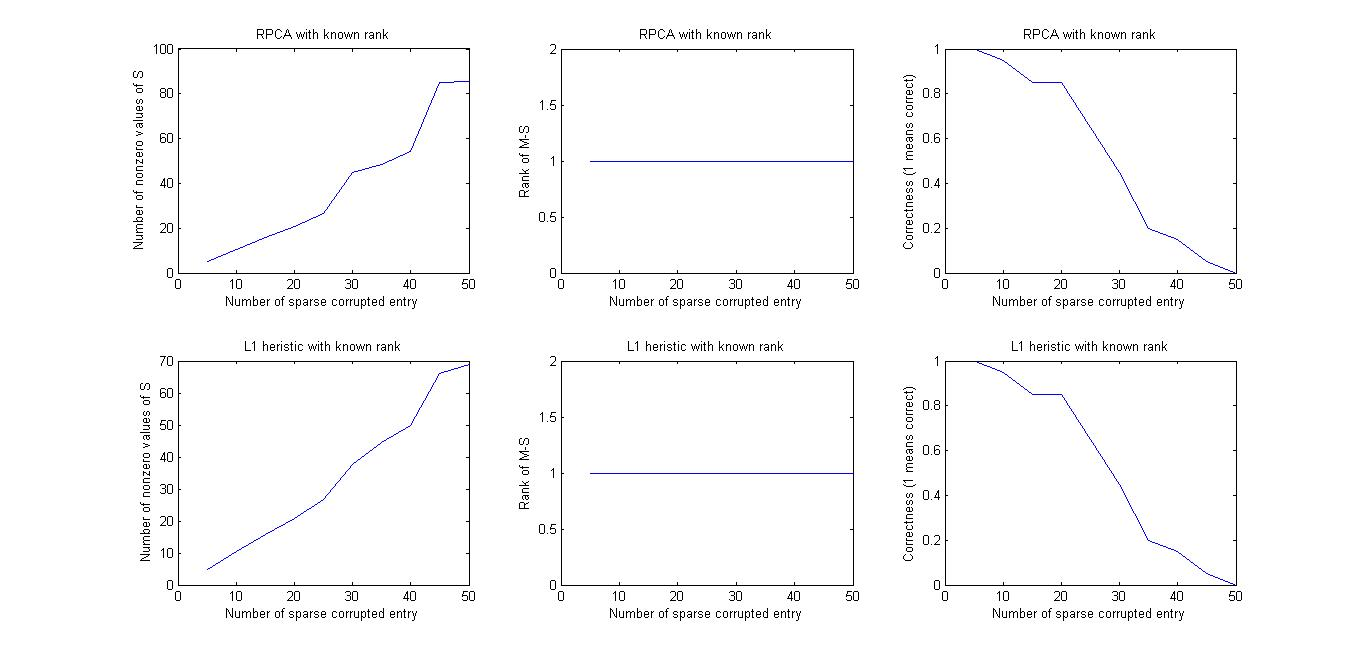
\includegraphics[width=16cm]{../figures/compare.jpg}
\end{figure}

